% --------------------------------------------------------------
% This is all preamble stuff that you don't have to worry about.
% Head down to where it says "Start here"
% --------------------------------------------------------------
 
\documentclass[12pt]{article}
 
\usepackage[margin=1in]{geometry}
\usepackage{graphicx}
\usepackage{amsmath,amsthm,amssymb}
\graphicspath{ {./} }
 
\newcommand{\N}{\mathbb{N}}
\newcommand{\Z}{\mathbb{Z}}
 
\newenvironment{theorem}[2][Theorem]{\begin{trivlist}
\item[\hskip \labelsep {\bfseries #1}\hskip \labelsep {\bfseries #2.}]}{\end{trivlist}}
\newenvironment{lemma}[2][Lemma]{\begin{trivlist}
\item[\hskip \labelsep {\bfseries #1}\hskip \labelsep {\bfseries #2.}]}{\end{trivlist}}
\newenvironment{exercise}[2][Exercise]{\begin{trivlist}
\item[\hskip \labelsep {\bfseries #1}\hskip \labelsep {\bfseries #2.}]}{\end{trivlist}}
\newenvironment{problem}[2][Problem]{\begin{trivlist}
\item[\hskip \labelsep {\bfseries #1}\hskip \labelsep {\bfseries #2.}]}{\end{trivlist}}
\newenvironment{question}[2][Question]{\begin{trivlist}
\item[\hskip \labelsep {\bfseries #1}\hskip \labelsep {\bfseries #2.}]}{\end{trivlist}}
\newenvironment{corollary}[2][Corollary]{\begin{trivlist}
\item[\hskip \labelsep {\bfseries #1}\hskip \labelsep {\bfseries #2.}]}{\end{trivlist}}

\newenvironment{solution}{\begin{proof}[Solution]}{\end{proof}}
 
\begin{document}
 
% --------------------------------------------------------------
%                         Start here
% --------------------------------------------------------------
 
\title{C Group Project Interim Report}
\author{Hoang Vu, Kaiyan Fan, Xuan(Tom) Zhao, Zelin(Daniel) Deng}

\maketitle

\noindent Over the past two weeks, we have progressively accomplished Part I of the ARM11 group project and have embarked on Part II. Below is a brief report on our work status:

\begin{itemize} %the first video is required (but you don't have to watch it first), you can choose the other 4 from the list on the Course Materials page
  
  %A statement on how you have split the work between group members and how you are coordinating your work.
  \item How we divide the workload:\\
  Before the release of the specification, we laid out basic guidelines including code styles and best git practices. We have also been organising biweekly meeting to composed detailed to-do lists and giving each other valuable feedback. Our primary strategy is to file an issue on GitLab for every task to avoid overlap of work, and then create a separate feature branch. During the development phase, we frequently comment and give advice to each other on the git issue. More importantly, as a merge request is issued, it is the whole group's responsibility to review it to ensure correctness and consistent code style. We also write unit tests in turn to ensure the correctness of each unit. In all, each of us has spent approximately equal amount of time between writing code and code reviews. Although our group has two members who are outside U.K., we take the advantage of the difference in timezone by working in turns.
  
  %A discussion on how well you think the group is working and how you imagine it might need to change for the later tasks.
  \item Summary and Improvements:\\
  We utilise git to enhance our workflow. The responses to comments and communications are generally fast. We have dedicated a large part of our time to compose a library of unit tests, written by all members, for each individual part of the project. This proved to be extremely successful as our program was almost perfect the first time we put it together. Furthermore, we proficiently use git as a tool of communication and organisation, thus we have not encountered, surprisingly, any major merge conflict. For further improvements, we should spend more time in the initial phase for part 2, laying out the structure in much greater depth. We should also specify all public interfaces across the module and write the header files before implementing each unit. This can reduce confusions during the development phase and avoid continuous modifications later.
  
  %How you have structured your emulator, and what bits you think you will be able to reuse for the assembler.
  \item The Structure of Our Emulator:\\
  We have agreed to use the structure for the emulator as shown in Figure~\ref{part1:UML} below. The UML diagram contains descriptions of each individual file as well as their dependencies. To make the folder structure cleaner, we put unit tests and header files in separate folders. We expect to reuse everything under \texttt{common} folder in the assembler module in Part II. We might also reuse some parts of the \texttt{logicunit} in order to calculate simple shifts and offsets in the assembly code in Part II, but this is still under discussion.
  \begin{figure}[!ht]
  \centering
  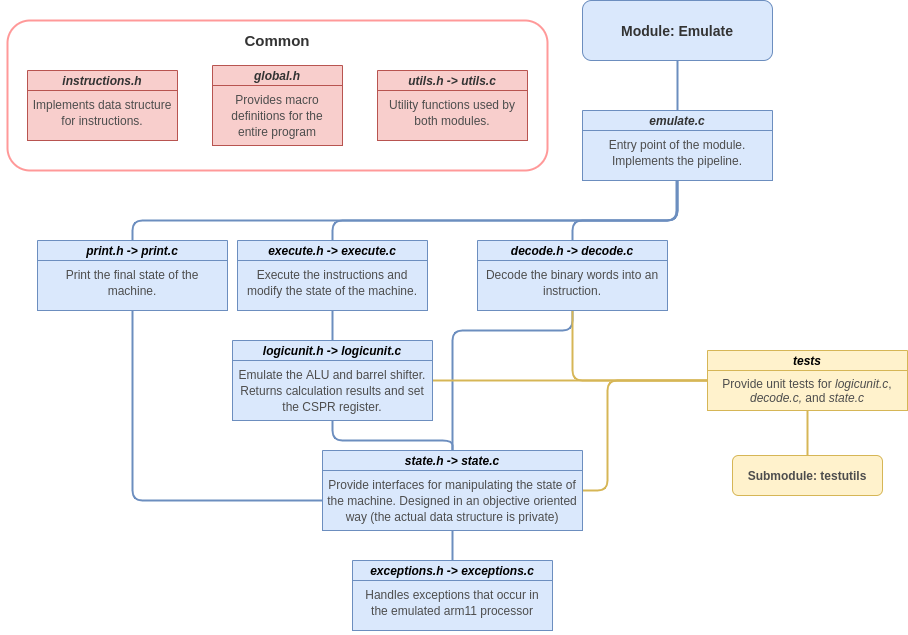
\includegraphics[scale = 0.5]{project_structure_interim.png}
  \caption{An UML Diagram of Emulator Structure}
  \label{part1:UML}
  \end{figure}
  
  %A discussion on implementation tasks that you think you will find difficult / challenging later on, and how you are working to mitigate these.
  \item Difficulties:\\
  One of the challenging tasks was to come up with a good representation of the instructions. Each of us had suggested at least one necessary change to the structure due to the need of decoding. The biggest issue was that changing the structure of instruction led to a chain of changes in other parts of the project as well, consuming a lot of time.\\
  The second challenge was to balance between writing an emulator and simulating an actual processor. Specifically, we tried to model the ALU and Barrel-Shifter in their raw form, which, at one point, resulted in a lot of boilerplate code.\\
  Another challenge was to deal with the endianness of data. The instructions are decoded by their \textit{big-endian} representations to improve readability, but data in memory are store in \textit{little-endian}. This is further complicated by the fact that UNIX systems are \textit{little-endian}. We overcame this challenge by repeated experimenting different strategies of dealing with the endianness.\\
  The weird behaviours of the program caused by mistakes in memory allocation also confused us a lot at debugging. However, thanks to unit tests, we managed to quickly identify the source of the problems. This proves the usefulness of unit tests, and we should keep writing them in part II.
  
  \item In conclusion, we have learned a lot in the first part of our project, from organisation skills to technical skills. We are very satisfied with our accomplishments so far.
\end{itemize}
 
% --------------------------------------------------------------
%     You don't have to mess with anything below this line.
% --------------------------------------------------------------
 
\end{document}
